\section{Dokumentengeschichte}
\begin{table}[h]
 \begin{tabular}{|l|l|p{4cm}|}
 \hline
 Zeitraum & PL/Autor(en) & Änderungen \\
 \hline
 Sommersemester 2017/18 & Khaled Halabieh 556290  & 
Imports
 
  \\
 \hline
 Wintersemester 2017/18 & Nabeel Smadi 556209 & 
Imports


  \\
 \hline
 \end{tabular}
 \caption{Dokumentengeschichte}
 \end{table}

\section{Aufgabe der Komponente}

Imports ist eine Webschnittstelle die zum Einbringen von Geometrien und historische Daten in das System dient.
Die Webschnittstelle nimmt durch post request Geojason und speichert die Daten auf PostGIS Datenbank als Geometrie.

\section{Architektur}

\subsection{Überlick}


\begin{figure}[h]
\centering
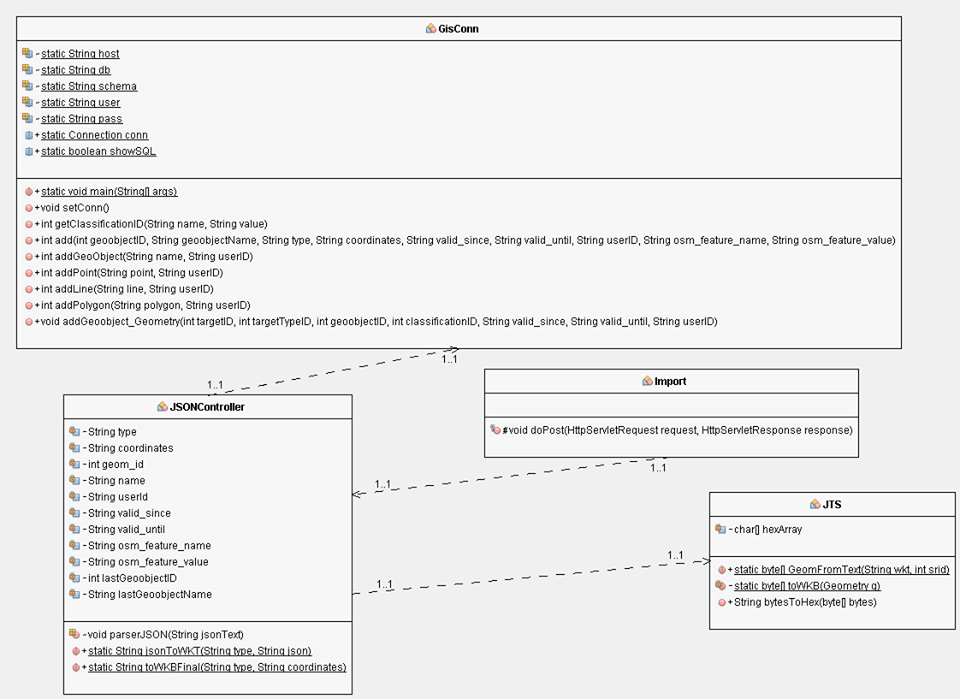
\includegraphics[page=1, width=127mm]{importer2/pic/UmlImporter.png}
\caption{UML Diagramm}
\label{fig:UmlImporter}
\end{figure}
%TODO Text zum Bild :)



\subsection{Schnittstellendefinitionen}

Das Projekt besteht auf eine Web Schnittstelle als Java Servlet die mit Rest Methoden arbeitet.
\subsection{genutztes Komponenten}

Das Projekt benutzt keine weitere Konponenten.
\section{Nutzung}
\subsection{Code}
Der Code befindet sich im Importer Repository.


\subsection{Deployment / Runtime}
Nach Compeilen wird ein WAR Datei erzeugt, diese WAR Datei wird durch Deployment auf GlassFish Server eingesetzt.

\section{Qualitätssicherung}
Das Projekt macht keine Validierung von Gson Datei, falls der Import nicht erfolgreich abgelaufen ist, wird ein Fehler Meldung angezeigt.


\section{Vorschläge / Ausblick}
Es fehlt noch die Validierung von JSON Datei, die den Nutzer zeigt, wo genau die Fehler liegen.